
%%%%%%%%% Section 2.4
\subsection{Comparison to Other Methods}\label{sec:othermethods}
We establish two comparisons: first to statistical Bayesian inversion \cite{Walpole, Berger, Complete}, the second to a measure-theoretic approach studied in \cite{BET+14}. 


\subsubsection{Statistical Bayesian Approach}

%If the quantity of interest is a single measurement, then the likelihoods and observed densities are identical.
%However, the quantity of interest may not necessarily just be the uncertainty in the measurement data, as we will see in later discussions. 
%For completeness, we define the alternative solution to the SIP below and compare the two frameworks under a simple linear map.

The ``statistical Bayesian'' (the term we use herein for clarity) formulation gives a updated density as:
\begin{equation}\label{eq:sb_post}
    \hat{\updated}\lam := \initial\lam \frac{L_\dspace (d | \param)}{ C },
\end{equation}
where we use $\hat{\updated}$ to distinguish the posterior from the updated density in \eqref{eq:update}, $L_\dspace$ is the likelihood function as a function of the output and the denominator $C$ is a \emph{normalizing constant}, chosen so that the updated density integrates to one, namely
\[
C = \int_\pspace \initial\lam L_\dspace(d | \param) \, d\param.
\]

It is important to note that the statistical Bayesian framework poses a different question for which a different answer is sought. 
Specifically, the problem analyzed by the statistical Bayesian approach is to determine a single ``true'' parameter that explains all of the observed data \cite{Smith, Concrete, Complete}.
In this framework, there is a different notion of consistency, referring to certain asymptotic properties of $\updated$ in the limit of infinite data \cite{Barron, Silverman}.
This is in contrast to the consistent Bayesian framework, where we seek a pull-back measure: a description of the uncertainty set that explains the variation in the observations under a given description of error.
We note that there are problems that one can formulate where the observed density corresponds directly to a normalized likelihood function familiar to Bayesian statisticians, as we demonstrate below. 

One difference that is immediately obvious between the two solutions is the use of normalizing constant $C$ in $\hat{\updated}$ not present in $\updated$, as discussed in Corollary~\ref{cor:int} above.
To illustrate the two approaches, we explore the impact of this difference in the example below, taken from \cite{BJW18}.

\begin{ex}
Consider
\begin{equation}
u(\param) = \param^p
\end{equation}
for $p$ chosen as either 1 or 5. 
For both approaches, the prior is given by $\initial \sim U[-1,1]$. 
In the consistent Bayesian approach, $\observed \sim \mathcal{N}(0.25,0.1^2)$.
In the statistical Bayesian framework, we take $d=0.25$ and assume an additive error noise model with distribution $\mathcal{N}(0,0.1^2)$ so that the likelihood, $L_\dspace(d | \param)$, matches the observed density as a function of $\param$.

When $p=1$, we have $\predicted = \frac{1}{2} = C$.
Since $\observed\q = L_\dspace(d|\param)$, the posterior and update agree on $\pspace$ (we show the push-forwards in the right plot of Figure~\ref{fig:comparison}). 
When $p=5$, the non-linearity of the model causes the push-forward of $\initial$ to be non-constant, so the two approaches yield differing solutions, as seen in the left plot of Figure~\ref{fig:comparison}).
The push-forward of the posterior associated with the statistical Bayesian framework is influenced by the push-forward of the prior in a way that the push-forward of the updated density avoids.

\begin{figure}\label{fig:comparison}

\begin{minipage}{.45\textwidth}
		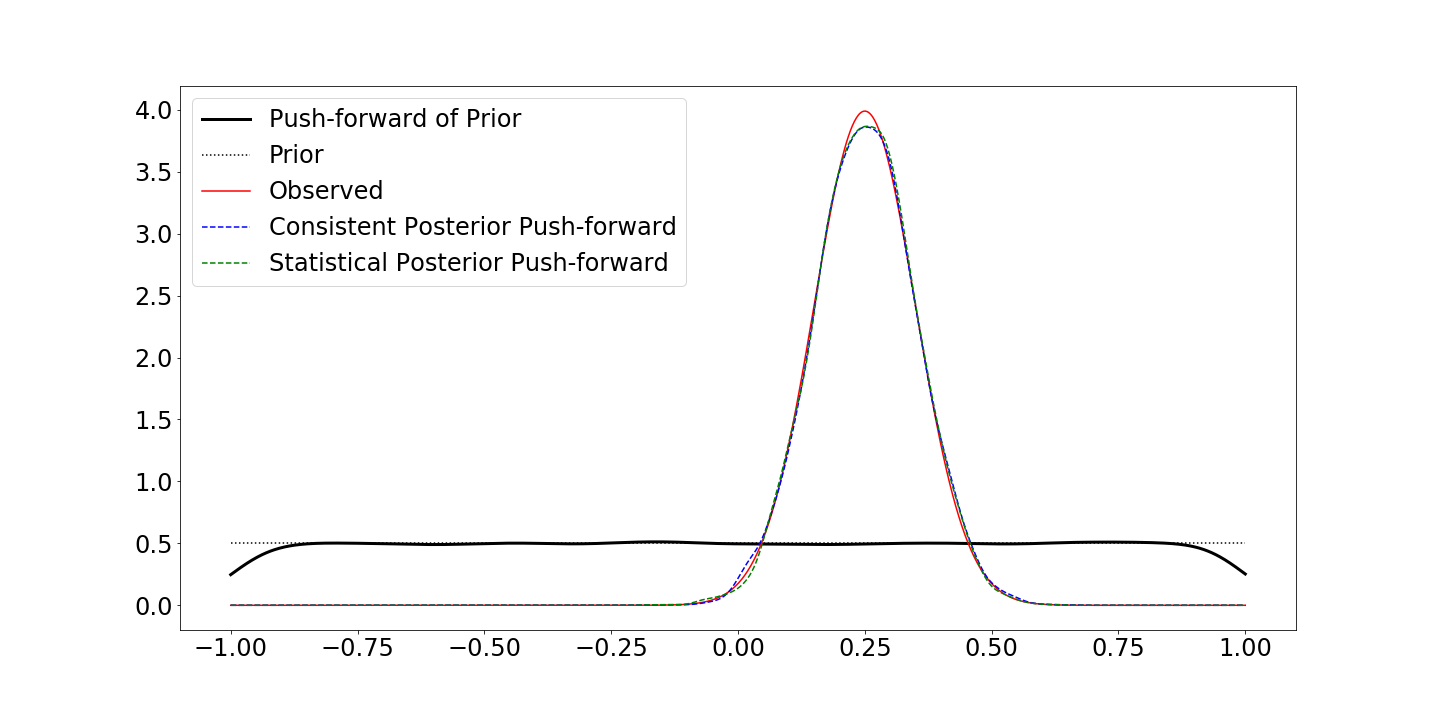
\includegraphics[width=\linewidth]{./images/comparison1}
\end{minipage}
\begin{minipage}{.45\textwidth}
		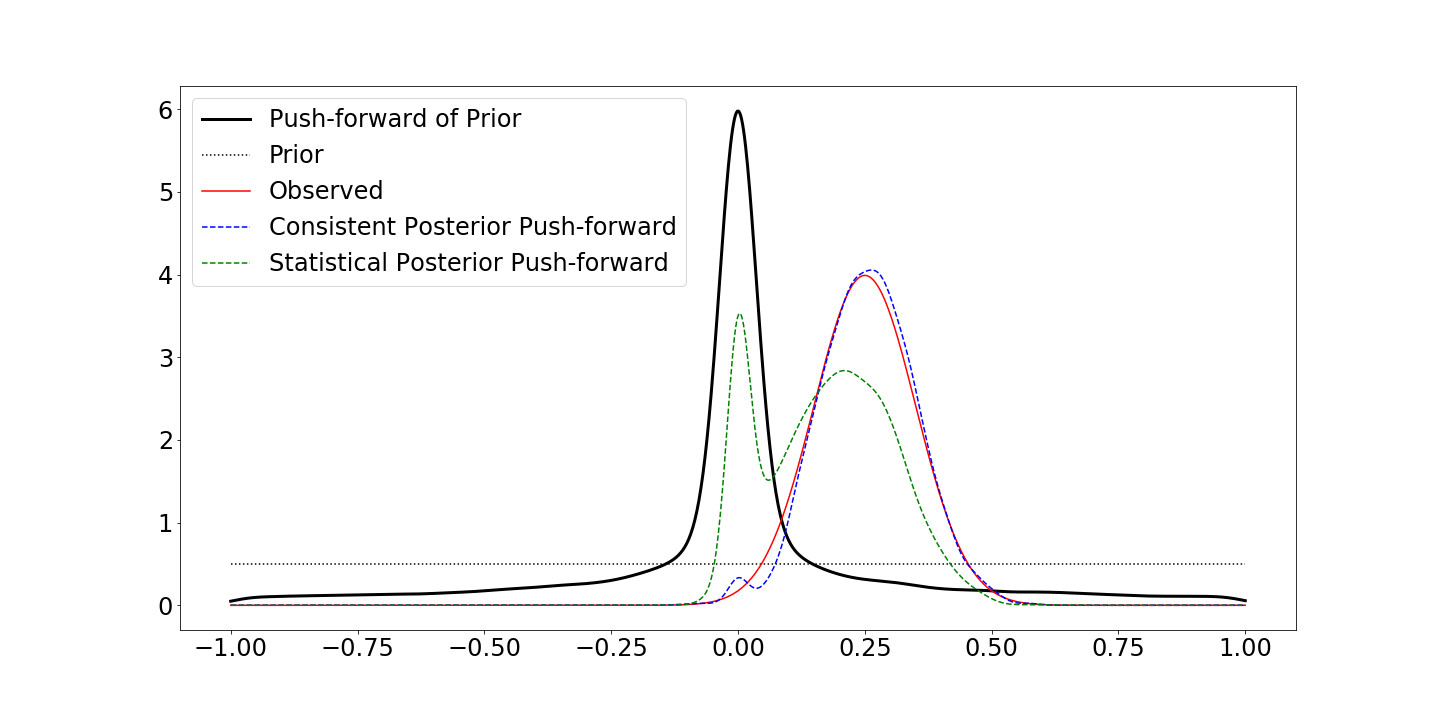
\includegraphics[width=\linewidth]{./images/comparison5}
\end{minipage}
\caption{In each plot, the black dotted line represents the prior while the solid line represents the push-forward of the prior. The push-forwards of the posterior and consistent updated density are shown as green and blue dotted lines, respectively. The observed density/likelihood is shown as a solid red line. (Left): $p = 1$, the push-forwards of the solutions are identical because a linear map results in a constant push-forward of a uniform prior. (Right): $p = 5$, the non-linearity of the map causes the solutions to be different and thus the push-forwards to also be different.}
\end{figure}

We can see in Figure~\ref{fig:comparison} that the two approaches pose different questions and thus yield different results. 
The consistent Bayesian framework seeks to recreate the observed density, which it does for both $p=1$ and $p=5$, but the statistical approach is a weighted sum of both the observed and the push-forward of the prior.
\end{ex}